\section{有限资源下的比较}
\label{sec:lossless-finite-resources}

前面的极限都在$n\to\infty$时成立，并且假定编码器知道真实的分布。实际选择编码方案时，块长有限，模型可能不准，码表要存储，编码要计算。本节在贯穿例上把各种方案放在同一组条件下比较：源分布相同，按每个源符号计算码长，解码要求分别写明。

\paragraph{几种方案的账本}
表~\ref{tab:lossless-comparison}列出贯穿例上的几种方案。平均码长一栏都按每源符号计；“最长码字”按一个编码单位（一个符号、一个块或整条消息）计；码本一栏是编码器与解码器需要共享的表的规模。

\begin{BookInlineTable}
 \centering
 \caption{贯穿例$p=(0.4,0.3,0.2,0.1)$上的几种编码方案，$H=1.846$。算术编码一行为图~\ref{fig:lossless-arith-length}中长$400$、长度已知的那条消息的实测值，码长小于消息自信息加$2$；定长块一行为图~\ref{fig:lossless-fixed-rate-error}中$R=1.95$、$n=100$的最优定长码。}
 \label{tab:lossless-comparison}
 \begin{tabular}{lcccc}
  \toprule
  方案 & 位/符号 & 最长码字 & 共享的表 & 错误概率\\
  \midrule
  定长$2$位 & $2$ & $2$ & 无 & $0$\\
  Huffman，$n=1$ & $1.900$ & $3$ & $4$项 & $0$\\
  Huffman，$n=2$ & $1.865$ & $6$ & $16$项 & $0$\\
  Huffman，$n=4$ & $1.853$ & $12$ & $256$项 & $0$\\
  Huffman，$n=6$ & $1.851$ & $19$ & $4096$项 & $0$\\
  算术编码 & $1.855$ & 随消息 & $4$个概率 & $0$\\
  定长块 & $1.95$ & $195$ & 排序规则 & $0.0015$\\
  \bottomrule
 \end{tabular}
\end{BookInlineTable}

从表中可以读出三点。第一，从$n=1$到$n=6$，块上Huffman码每符号只省下$0.049$位，码表却从$4$项增长到$4096$项，最长码字从$3$位增长到$19$位：越接近熵，每一点改进越贵。第二，算术编码只需共享四个概率，就达到了与$n=6$的块Huffman码相当的每符号码长；代价是每个符号要做乘法和区间比较，并且要处理有限精度。第三，定长块编码的码字最整齐，但要接受正的错误概率，不能用于必须逐条还原的场合。

\paragraph{码本的描述代价}
若编码器与解码器事先没有共享码表，码表本身也要传送。Huffman码由码长完全决定：把码长按从短到长排好，用第~\ref{sec:lossless-kraft}小节Kraft不等式充分性证明中的方法分配码字，得到的前缀码称为规范码，解码器只需知道每个块的码长。块长为$n$时要传送$4^n$个码长，每个码长用几位表示，总共是$4^n$乘以一个常数的位数。若消息只有$N$个符号，这一开销摊到每个符号上是$4^n/N$量级，块长增大带来的不到$1/n$位的收益，很快被它抵消。算术编码只需传送模型的四个概率（或模型的更新规则），描述代价与块长无关。

\paragraph{计算代价}
块上Huffman码的构造需要对$4^n$个块排序合并，计算量$O(4^n\cdot n)$；编码时查表，解码时在码树上逐位行走。算术编码不需要构造码表，每读一个符号做常数次乘法与比较，解码时要在累积概率表中找到$v$所在的子区间，字母表较大时用二分查找。两者都是每个源符号常数量级的工作，但Huffman码的常数随块长指数增长，算术编码的常数与消息长度无关。

\paragraph{模型失配的代价}
设计编码时用的分布$q$称为模型，信源的真实分布是$p$，两者可能不同。码长是按$q$设计的，平均码长却要按实际出现的频率，即按$p$加权。定理~\ref{thm:lossless-entropy-bound}证明中的分解在这里给出精确的账目。

\begin{theorem}[失配的Shannon码]
\label{thm:lossless-mismatch}
设$p,q$是$\mathcal{X}$上的概率质量函数，各$p(x)>0$、$q(x)>0$，且$q(x)<1$对每个$x$成立。按模型$q$取码长$\ell(x)=\lceil-\log_2q(x)\rceil$的前缀码，在真实分布$p$下的平均码长满足
\begin{equation}
 H(p)+D_{\mathrm{KL}}(p\Vert q)\leq\sum_xp(x)\ell(x)<H(p)+D_{\mathrm{KL}}(p\Vert q)+1 ,
 \label{eq:lossless-mismatch}
\end{equation}
其中$H(p)$是$p$的熵。
\end{theorem}

\begin{proof}
码长满足Kraft不等式，理由同定理~\ref{thm:lossless-entropy-bound}，所以这样的前缀码存在。对每个$x$，
\[
 -\log_2q(x)=-\log_2p(x)+\log_2\frac{p(x)}{q(x)} .
\]
按$p$加权求和，右边的平均是$H(p)+D_{\mathrm{KL}}(p\Vert q)$。而$-\log_2q(x)\leq\ell(x)<-\log_2q(x)+1$，乘$p(x)$求和即得式~\eqref{eq:lossless-mismatch}。
\end{proof}

所以模型失配的代价是KL散度$D_{\mathrm{KL}}(p\Vert q)$：按错误的概率分配码长，每符号平均多付这么多位。左侧的不等式说明这部分损失无法靠取整挽回；它与整数码长的冗余是两笔不同的账。

图~\ref{fig:lossless-mismatch}在贯穿例上让模型从$p$逐渐变到反序的$r=(0.1,0.2,0.3,0.4)$，即$q_t=(1-t)p+tr$。$t=0$时模型准确，Huffman码平均$1.9$位；$t=1$时按$r$设计的Huffman码给$a$三位、$d$一位，按真实概率加权，
\[
 0.4\times3+0.3\times3+0.2\times2+0.1\times1=2.6 ,
\]
比准确模型多$0.7$位，比定长码还差。此时$D_{\mathrm{KL}}(p\Vert r)=0.658$，Shannon码平均$3.1$位，落在式~\eqref{eq:lossless-mismatch}给出的$[2.505,3.505)$中。另一个特例是均匀模型：码长都是$2$，平均码长$2$恰好等于
\[
 H(p)+D_{\mathrm{KL}}(p\Vert u)=1.846+0.154 .
\]

\begin{BookInlineFigure}
 \centering
 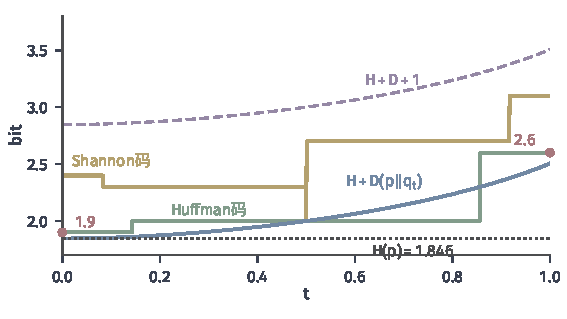
\includegraphics[width=96mm]{figures/07-probability/05-source-coding/matplotlib/lossless-mismatch/figure.pdf}
 \caption{模型失配。真实分布$p=(0.4,0.3,0.2,0.1)$，设计模型$q_t=(1-t)p+t\,r$，$r=(0.1,0.2,0.3,0.4)$。纵轴为按$p$计算的平均码长：黄线为按$q_t$设计的Shannon码，绿线为按$q_t$设计的Huffman码；蓝线为$H(p)+D_{\mathrm{KL}}(p\Vert q_t)$，紫色虚线为再加$1$，灰色点线为$H(p)$。红点为两端的Huffman码平均码长。}
 \label{fig:lossless-mismatch}
\end{BookInlineFigure}

图中Huffman码的曲线是阶梯形：模型稍有偏差时，码长的整数取值往往不变，平均码长也不变；偏差累积到改变码树时才跳一级。在$t$约从$0.5$到$0.86$之间，按$q_t$设计的Huffman码甚至落在蓝线下方，这并不矛盾：式~\eqref{eq:lossless-mismatch}只约束Shannon码，任何码的平均码长只受$H(p)$约束。

\paragraph{失配与不一致是两回事}
模型失配时，编码器与解码器用同一个$q$，码仍然唯一可译，每条消息都正确还原，只是平均更长。另一种错误是两端不一致：编码器与解码器用了不同的码表或不同的概率。这时码长没有变，解码结果却错了。

两个例子都来自本章的码表。第~\ref{sec:lossless-model}节的码表中$c\mapsto110$、$d\mapsto111$，第~\ref{sec:lossless-huffman}小节Huffman过程得到的码表中$c\mapsto111$、$d\mapsto110$，两者平均码长相同。若编码器用前者把$abac$编成$0100110$，解码器却用后者，读出的是$abad$。算术编码也一样：编码器按$p=(0.4,0.3,0.2,0.1)$把$abac$编成$00110010$，若解码器误用$(0.3,0.4,0.2,0.1)$，则从$v=0.1953$逐步读出
\[
 a,\quad b,\quad c,\quad c ,
\]
得到$abcc$。

所以评价一个方案要分开两件事：在两端一致的前提下，模型偏离真实分布会使平均码长增加$D_{\mathrm{KL}}(p\Vert q)$左右；两端不一致则破坏可解码性，与平均码长无关。前者靠更好的模型改进，后者要靠严格共享的规则（码长表、符号顺序、概率与取整方式）来避免。
